%% [ADS 4-2005] Template file for 40in x 30in landscape poster
%%
%%
%%
%%
%% [ADS 4-2005] what follows here is obsolete I believe.
%%-------------------------------------------------------------------------
%% Written by Graeme, 2001-03 based on Norman's original microlensing
%% poster.
%%
%% $Id: poster-template-landscape.tex,v 1.1 2001/07/02 17:23:32 norman Exp $
%%
%% Default mode is landscape, which is what we want, however dvips and
%% a0poster do not quite do the right thing, so we end up with text in
%% landscape style (wide and short) down a portrait page (narrow and
%% long). Printing this onto the a0 printer chops the right hand edge.
%% However, 'psnup' can save the day, reorienting the text so that the
%% poster prints lengthways down an a0 portrait bounding box.
%%
%% 'psnup -w85cm -h119cm -f poster_from_dvips.ps poster_in_landscape.ps'
%%
%%-------------------------------------------------------------------------
%% Modified by Ronald Kumon, 06-2002 to incorporate a framebox border,
%%   add acknowledgments line at bottom, and change locations of logos
%%
%% Modified by Anand D. Sarwate 04-2005 to specialize to the UC Berkeley 
%%   EECS Wireless Foundaions conference poster template and for different
%%   paper sizes


%% [ADS 4-2005] latex --> dvips --> ps2pdf works just fine for me.
%%
%% To preview using xdvi:
%% 
%% $ xdvi -paper 1188x840mm -s 24 -nopostscript poster.dvi
%%
%% To convert dvi to Postscript:
%%
%% $ dvips -Ppdf -G0 -o poster.ps poster.dvi
%%
%% The dvips options are:
%% Ppdf: use the PDF printer configuration file
%% G0  : shift lower characters to higher position 
%%       (splits ligatures when using Times-Roman font)
%%
%% To convert Postscript to PDF:
%%
%% $ pstill -c -giptCQ -w 3368 -h 2378 -o poster.pdf poster.ps
%% ($ pstill -c -iptCQ -w 3225 -h 2378 -o poster.pdf poster.ps)
%%
%% Note that the pstill options are
%% c:  compression (more c's give more compression; up to four)
%% g:  take size from Postscript file
%% p:  include all fonts as partial fonts
%% i:  include all non-standard fonts
%% t:  map graphics transfer functions from PostScript to PDF. 
%% C:  use RGB color map
%% w:  width in points (1/72 inch) for 1188 mm
%% h:  height in points (1/72 inch) for 839 mm
%% Q:  take embedded fonts from PSFonts directory, not Postscript file
%% Note also that the -w and -h options need to be included else
%% some of the Postscript figures may not be displayed (particularly
%% those converted using fig2dev), even if the -g option is specified.
%% Also, the newest version of pstill (1.55.91) does not deal well with 
%% slanted Times Roman font; use italics or the older version (1.55.3). 
%%-------------------------------------------------------------------------


\documentclass{article}
%% [ADS 4/2005]  The template here does NOT make use of the 'slides'
%% option of Kumon in the interest of creating a more readable document
%% -- suggestions for how to make a backup style on separate sheet is
%% given in the text.
%%

%% If you want to number equations, set the equation number counter to zero.
%\setcounter{secnumdepth}{0}









%%%%%%%%%%%%%%%%%%%%%%%%%
%%% PACKAGE INCLUSION %%%
%%%%%%%%%%%%%%%%%%%%%%%%%

%% AMS packages for special symbols, etc
\usepackage{amsmath,amssymb}
\usepackage[inline]{enumitem}

%% This package gives you coloured text and various other simple
%% graphics hacks.  For details, see documentation in 
%% in /usr/local/teTeX/texmf/doc/generic/pstricks/*
\usepackage{pstricks}
\newrgbcolor{darkblue}{0.1 0.1 0.5}

%% The textpos package is necessary to position textblocks at arbitary 
%% places on the page.  Use showboxes option to show outlines of textboxes.
\usepackage[absolute]{textpos}
%\usepackage[absolute,showboxes]{textpos}

%% Package to include graphics.  
\usepackage{graphicx}
%% Define path for figures -- for safety, keep the last /
\graphicspath{{/your/figure/directory/here/if/any/}
{/an/second/directory/path/can/go/here/}}

%% Wrap text around figures
%\usepackage{wrapfig}

%% Use Times font instead of Computer Modern -- this gives better
%% appearance when resizing to large sixes.
%% Note that without the ``G0'' in the dvips conversion, 
%% all character combinations that will normally result in 
%% ligatures will have to be hacked to display properly.  For example, 
%%     fi --> \mbox{f}\mbox{i}
%% Other characters may also fail.  In addition, the Mathtimes font 
%% set should really be used for mathematics, but unfortunately they 
%% are only proprietary.  (The Computer Modern fonts may still look OK.)
\usepackage{times}

%% These colors are tried and tested for titles and headers. Don't
%% over use color!
%\usepackage[usenames]{color} % commented by Karol Kozioł
\usepackage{xcolor}
\definecolor{DarkBlue}{rgb}{0.1,0.1,0.5}
\definecolor{Black}{rgb}{0.0,0.0,0.0}
\definecolor{Red}{rgb}{0.9,0.0,0.1}
\definecolor{DarkBlue2}{rgb}{0.00,0.08,0.6}
\definecolor{DarkRed2}{rgb}{0.6,0.00,0.08}
\definecolor{DarkGreen2}{rgb}{0.00,0.6,0.08}


%% Load shadow box package
%\usepackage{shadow}

%% This loads font sizes in style file a0size
\usepackage{a0size}





%%%%%%%%%%%%%%%%%%%%%%%%%%%%%%%% 
%%% NEW COMMAND DEFINTITIONS %%%
%%%%%%%%%%%%%%%%%%%%%%%%%%%%%%%%

%% See documentation for a0poster class for the size options here
%%    \normalsize will produce smaller type that might look too small
%%    \large will produce larger type
%% Feel free to modify if you want a different look
\let\Textsize\normalsize
%\let\Textsize\large
\def\RHead#1{\noindent\hbox to \hsize{\hfil{\LARGE\color{DarkBlue} #1}}\bigskip}
\def\LHead#1{\noindent{\LARGE\color{DarkBlue} #1}\bigskip}
\def\CHead#1{\begin{center}\noindent{\LARGE\color{DarkBlue} #1}\end{center}}
\def\Subhead#1{\noindent{\large\color{DarkBlue} #1}\bigskip}
\def\Title#1{\noindent{\textbf{\Huge\color{DarkBlue} #1}}}




%%%%%%%%%%%%%%%%%%%%%%%%%%%%%
%%% GLOBAL LAYOUT OPTIONS %%%
%%%   NUMBER OF COLUMNS   %%%
%%%%%%%%%%%%%%%%%%%%%%%%%%%%%

%% Set paper size
%% Depending on the conference, the posterboard size may be different.
%% This template was based on an ISO standard A0, which is in use everywhere
%% except for the United States.  A0 paper is  46.81 in x 33.11 in.
%% Depending on the posterboard size and the printer, you may need to 
%% change the widths and margins here.  Text width and height are set
%% in terms of paper width and height -- you can change margins here.
\setlength{\paperwidth}{40in}
\setlength{\paperheight}{30in}
\setlength{\textwidth}{36in}    %% paperwidth - (3in)
\setlength{\textheight}{26in}   %% paperheight - (3in)
\special{papersize=\the\paperwidth,\the\paperheight}
\typeout{Paper width and height are \the\paperwidth and \the\paperheight}
\typeout{Text width and height are \the\textwidth and \the\textheight}
%% Margins
\setlength{\headheight}{0cm}
\setlength{\headsep}{0cm}
\setlength{\topmargin}{1in}
\setlength{\topskip}{0cm}
\setlength{\oddsidemargin}{1in}
\setlength{\evensidemargin}{0in}
%% Font sizes
\renewcommand{\tiny}{\fontsize{12}{14}\selectfont}
\renewcommand{\scriptsize}{\fontsize{14.4}{18}\selectfont}   
\renewcommand{\footnotesize}{\fontsize{17.28}{22}\selectfont}
\renewcommand{\small}{\fontsize{20.74}{25}\selectfont}
\renewcommand{\normalsize}{\fontsize{24.88}{30}\selectfont}
\renewcommand{\large}{\fontsize{29.86}{37}\selectfont}
\renewcommand{\Large}{\fontsize{35.83}{45}\selectfont}
\renewcommand{\LARGE}{\fontsize{43}{54}\selectfont}
\renewcommand{\huge}{\fontsize{51.6}{64}\selectfont}
\renewcommand{\Huge}{\fontsize{61.92}{77}\selectfont}
\newcommand{\veryHuge}{\fontsize{74.3}{93}\selectfont}
\newcommand{\VeryHuge}{\fontsize{89.16}{112}\selectfont}
\newcommand{\VERYHuge}{\fontsize{107}{134}\selectfont}
%% skip lengths
\setlength{\smallskipamount}{6pt plus 2pt minus 2pt}
\setlength{\medskipamount}{12pt plus 4pt minus 4pt}
\setlength{\bigskipamount}{24pt plus 8pt minus 8pt}
\setlength{\abovecaptionskip}{25pt}
\setlength{\belowcaptionskip}{0pt}
\setlength{\abovedisplayskip}{25pt plus 6pt minus 15 pt}
\setlength{\abovedisplayshortskip}{0pt plus 6pt}
\setlength{\belowdisplayshortskip}{13pt plus 7pt minus 6pt}
\setlength{\belowdisplayskip}{\abovedisplayskip}

%% Set up the grid
%%
%% Note that [40mm,40mm] is the margin round the edge of the page
%% it is _not_ the grid size. That is always defined as 
%% PAGE_WIDTH/HGRID and PAGE_HEIGHT/VGRID. In this case we use
%% 46 x 26. This gives us 4 columns of width 10 boxes, with a gap of
%% width 2 in between them.  There are 26 vertical boxes.
%%
%% (Note however that texblocks can be positioned fractionally as well,
%% so really any convenient grid size can be used.)
%%
\TPGrid[40mm,40mm]{46}{26}      % 4 cols of width 10, plus 3 gaps width 2

%% Text layout parameters
\parindent=0pt
\parskip=0.5\baselineskip





%%%%%%%%%%%%%%%%%%%%%
%%% THEOREMS, ETC %%%
%%%%%%%%%%%%%%%%%%%%%
\newtheorem{thm}{Theorem}

\usepackage[numbers,sort&compress]{natbib}
\renewcommand{\bibsection}{}




%%%%%%%%%%%%%%%%%%%%%%%%%%%%
%%% DOCUMENT BEGINS HERE %%%
%%%%%%%%%%%%%%%%%%%%%%%%%%%%

%% The basic format of the poster is to create text boxes with the
%% various things you want to display.  You can then play around 
%% with how to lay thing out.  In the old version of this template,
%% the content was always provided with alternatives suitable for
%% printing on sheets of paper (resizing fonts, images, etc).  I
%% think that's too confusing to read.  The old layout was:
%%     \ifposter
%%          some poster commands go here
%%     \else
%%          an alternative style here in case you are printing on
%%          regular sheets of paper
%%     \fi
%% One option is to make the entire poster and then wrap it in an \ifposter
%% and then make all the slides separately.  This seems to be easier
%% if your poster is not much like a bunch of 8.5x11 sheet tacked together
%% in the first place.
\begin{document}

%% Do not put page numbers at the bottom of the page for poster
\pagestyle{empty}



%% Declare proper hyphenation
\hyphenation{equi-bi-ax-i-al}
\hyphenation{in-fin-i-tes-i-mal}


%% Border and background options -- you can make up others if you
%% like.  These all use the pstricks package.
%% DRAW A BLUE BORDER AROUND THE POSTER USING PSTRICKS
\psset{linewidth=0.5cm}
% Sets up lengths for frame
\newlength{\frameleft}
\newlength{\frameright}
\newlength{\frametop}
\newlength{\framebottom}
\setlength{\frameleft}{-1in}
\setlength{\frameright}{\textwidth}
\addtolength{\frameright}{1in}
\setlength{\frametop}{1in}
\setlength{\framebottom}{-\textheight}
\addtolength{\framebottom}{-1in}
% Draws a blue frame
%\psframe[linecolor=darkblue,cornersize=absolute,linearc=2]
%(\frameleft,\framebottom)(\frameright,\frametop)% need to overlay EOSMLS
%\psline{->}(0cm,0cm)(\textwidth,-\textheight)
%   *** End code to draw border *** 

%% USE A COLORED BACKGROUND FOR THE ENTIRE POSTER
%% [ADS 4-2005] THIS OPTION IS NOT SUPPORTED YET
%\newrgbcolor{gradbegin}{0.3 0.5 0.7}
%\newrgbcolor{LightBlue}{0.7 0.7 1.0}
%\psframe[fillstyle=solid,fillcolor=LightBlue](\frameleft,\framebottom)(\frameright,\frametop)



%% Adjust spacing in long displayed mathematical formulas to tighten them up
\setlength{\abovedisplayskip}{0.75\abovedisplayskip}
\setlength{\belowdisplayskip}{0.75\belowdisplayskip}



%% Understanding textblocks is the key to being able to do a poster in
%% LaTeX. The first argument gives the block width in grid cells, the
%% second gives the positioning on the grid.
%%
%% NOTE:  You will have to do a lot of previewing to get everything
%% in the right place.
%%
\begin{textblock}{46}(00,00)
\begin{center}
\Title{Molten Salt Microreactor Controller Design Decisions}
\end{center}
\end{textblock}

\begin{textblock}{46}(00,01)
\begin{center}
\LHead{Sam J. Root*, Michael McKellar}\\
\LHead{\textit{*sjroot@uidaho.edu}}
\end{center}
\end{textblock}


%% UCB EECS logo on left, Wireless Foundations Logo on right
\begin{textblock}{8}(00.5,0.25)
\begin{center}

\includegraphics[height=4cm]{ne-logo}
\end{center}
\end{textblock}

\begin{textblock}{8}(38,0.25)
\begin{center}
%\includegraphics[height=5cm]{wifound.eps} % modified by Karol Kozioł
\includegraphics[height=4cm]{caes}
\end{center}
\end{textblock}


\begin{textblock}{42}(01,02.5)
\begin{center}
\rule{1200pt}{7pt}
\end{center}
\end{textblock}



%% Left Column
\begin{textblock}{10}(00,02.5)
\CHead{Introduction}            %% \CHead creates a centered title
\begin{itemize}
\item Natural circulation molten salt reactors have two passive feedback mechanisms that must be considered when designing a controller
\item Temperature reactivity caused by heavy-metal thinning and doppler broadening \cite{PetersonMS}
\item Flow reactivity caused by the advection of delayed neutron precursors out of core \cite{CarterPHD}
\end{itemize}
\end{textblock}



\begin{textblock}{10}(00,6.5)
\CHead{Thought Experiment}
Start design process by investigating dynamics associated with anticipated transients:
\begin{itemize*}
    \item Natural circulation flow mode
    \item Passive feedback mechanisms
    \item Transport delays
\end{itemize*}\\
Conduct a thought experiment
\begin{itemize*}
    \item Power step increase 
    \item Core set-point instantly equal to heat exchanger power demand
    \item Ideal controller which produces rapid load following and disturbance rejection
\end{itemize*}

\begin{center}
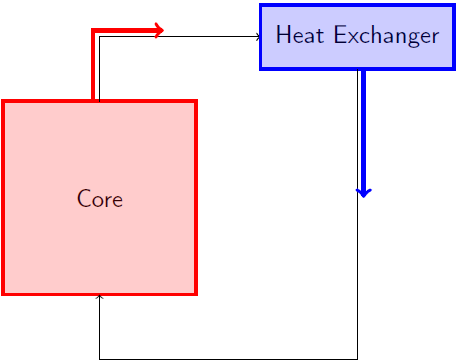
\includegraphics[width=4.8in]{Thought-1.png}

Immediately, the core produces more power and the heat exchanger rejects more power. This results in a higher flow-rate and a negative flow reactivity insertion

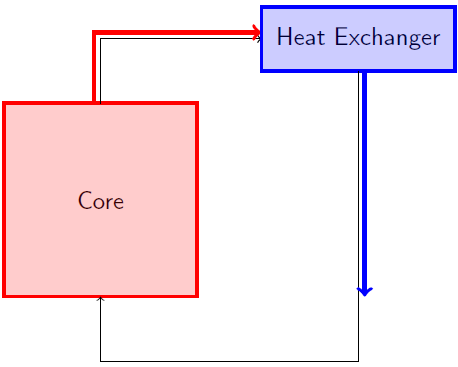
\includegraphics[width=4.8in]{Thought-2.png}

When the hot salt from the core reaches the heat exchanger, the additional power is delivered and the downcomer returns to its normal temperature

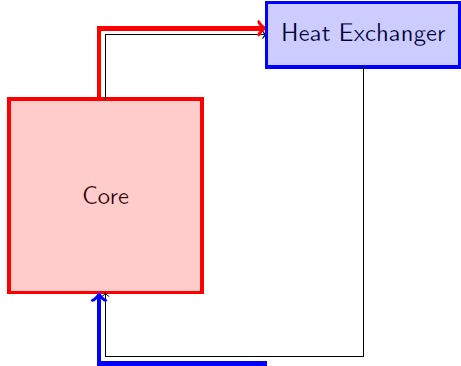
\includegraphics[width=4.8in]{Thought-3.png}

When the cold salt from the heat exchanger arrives in the core, this is a positive temperature reactivity insertion, followed by a negative temperature reactivity insertion when the normal temperature salt arrives
\end{center}
\end{textblock}

%Middle Columns
\begin{textblock}{22}(12,3.5)
    \CHead{Molten Salt Microreactor Control Loop}
    \begin{center}
    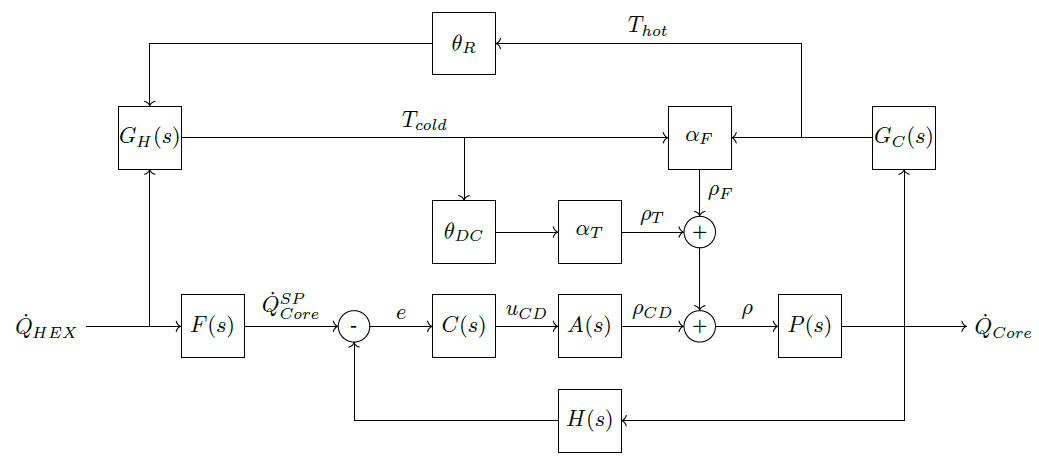
\includegraphics[width=18in]{Loop.png}

    Typical feedback loop with a pre-filter, with the addition of the passive feedback mechanisms. The core ($\dot{Q}_{Core}$) and heat exchanger ($\dot{Q}_{HEX}$) powers go through the respective temperature dynamics ($G_C$ and $G_H$) and time delays for the riser ($\theta_R$) and downcomer ($\theta_{DC}$) before being converted to reactivity by the temperature($\alpha_T$) and flow ($\alpha_F$) feedback mechanisms. The passive reactivity feedback is combined with the control drum reactivity ($\rho_{CD}$) and fed into the reactor dynamics ($P(s)$).

    \end{center}
    \end{textblock}


\begin{textblock}{10}(12,14.5)
\CHead{Pre-Filter}
\begin{equation*}\label{eqn:prefilter}
    F(s)=\frac{1}{\tau_F s+1}    
\end{equation*}

Pre-filters are unity gain transfer functions that provide inertia against rapid changes. A pre-filter that reshapes the core set-point after a change to heat exchanger demand will make the initial hot edge more gradual. This will allow the temperature profile to equilibrate more quickly rather than settling into bi-stable resonance. Proper tuning of the pre-filter time-constant will allow the reactivity oscillations to decay more quickly. 

\begin{center}
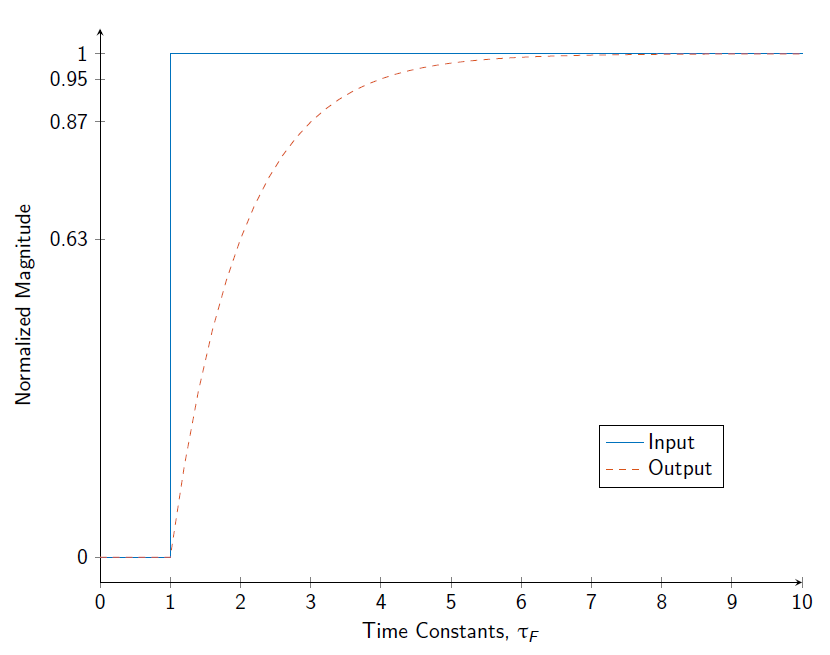
\includegraphics[width=8in]{Prefilter.png}
\end{center}
\end{textblock}

\begin{textblock}{10}(24,14.5)
\CHead{Dead-band}
A dead-band is a type of piecewise function where the output is null for inputs surrounding zero ($\pm \delta$) but has some other value for inputs with greater magnitude. It is common in thermostatic controls (where the furnace in a home only turns on when the temperature inside is sufficiently far from the setpoint). In process control, it is common for a controller gain ($K_C$) to be dead-banded to avoid swift periodic actuation.

\begin{equation*}
    K_C=
        \begin{cases}
            K_C & \text{if } e < -\delta \\
            0 & \text{if } -\delta < e < \delta \\
            K_C & \text{if } e > \delta 
        \end{cases}
\end{equation*}\\


    Previous work \cite{CarterPHD} has shown that the passive feedback mechanisms (temperature and flow reactivity) are capable of autonomous load following for small transient, though not at the level of performance that may be required in certain applications. Still, this provides the opportunity to minimize fine and rapid actuation while dampening oscillations by using a dead-band; the `ringing out' of minor perturbations could be left to the passive feedback mechanisms after the active feedback controls the bulk of the power change.


\end{textblock}

%Right Column

\begin{textblock}{10}(36,02.5)
\CHead{PID Controller}
The controller output ($u$) is often determined by a PID equation, which considers the instantaneous, cumulative, and predictive error. This equation has three terms:
\begin{enumerate}
\item Proportional control term. The control output is manipulated in proportion to the error defined by the proportional gain constant ($K_P$).   
\item Integral control term, which considers the historical cumulative error in an effort to eliminate steady-state offset that a P-Only controller may exhibit. As the process variable settles around the set-point, the cumulative error approaches a constant value and the effect of the integral controller diminishes.
\item Derivative control term, which estimates the time rate of change of the error to dampen overshoot. This mechanism is sometimes referred to as anticipatory control. 
\end{enumerate}

A nuclear reactor is controlled by manipulating the criticality of the core, making it supercritical to increase the power, and subcritical to decrease. This is a highly time dependant exponential control mechanism. The derivative controller time constant will need to be carefully tuned to minimize the likelihood of significant overshoot following a power transient


\begin{equation*}\label{eqn:pid}
    u(t) 
    = \underbrace{K_P e(t)}_{\text{Proportional}} 
    + \underbrace{K_I \int_0^t e(t)dt}_{\text{Integral}} 
    + \underbrace{K_D \frac{de(t)}{dt}}_{\text{Derivative}}
\end{equation*}
\end{textblock}


\begin{textblock}{10}(36,15)
\CHead{Future Work}
\begin{itemize}
    \item Neutronics modeling will be conducted to characterize the actuator-control reactivity curve ($A(s)$)
    \item Finite-element process simulation will be conducted to characterize the heat exchanger ($G_H(s)$), core ($G_C(s)$), and overall reactor ($P(s)$) dynamics
    \item A gain/bias schedule will be developed to account for the fact that more control reactivity is required to make the reactor go critical later in the fuel lifetime
    \item Poison reactivity from the build-up of xenon-135 may be accounted for using a Bode-Step controller \cite{Roberson}
\end{itemize}



\end{textblock}


\begin{textblock}{10}(36,20.5)
\CHead{References}
\bibliographystyle{../nsf}
\bibliography{../References}
\end{textblock}



\begin{textblock}{46}(00,26)
\begin{center}
{\footnotesize Acknowledgments: This work and my coursework in pursuit of an M.S. in Nuclear Engineering is being completed under a Graduate Fellowship funded by Nuclear Regulatory Commission }
\end{center}
\end{textblock}

\end{document}
